%!TEX program = xelatex

\documentclass{article}
\usepackage{algorithm}
\usepackage{algorithmic}
% \usepackage[utf8]{inputenc}
%\usepackage[UTF8]{ctex}
\usepackage{indentfirst}
\usepackage{lmodern}% http://ctan.org/pkg/lm
\usepackage{setspace}
\usepackage{verbatim}
\usepackage{amsmath}%数学
\usepackage{amsthm}%数学定理、证明
\usepackage{graphicx}%graphicx基于graphics,更方便
% \usepackage{subfig}%图像
\usepackage{subfigure}
\usepackage{booktabs}%表格
\usepackage{tabularx}%表格
\usepackage{multirow}
\usepackage{multicol}
\usepackage{listings}
\usepackage{relsize}
\usepackage[usenames]{color}   
\usepackage{fontspec}

%\usepackage{colortbl}%表格颜色
\usepackage[table]{xcolor}
\usepackage{array}
\usepackage[rightcaption]{sidecap}
\usepackage{hyperref}
\usepackage{float}
\hypersetup{
colorlinks=true,
linkcolor=black
}%解决目录红框问题
\lstset{
         language = vhdl, numbers=left, 
         numberstyle=\tiny,keywordstyle=\color{blue!70},
         commentstyle=\color{red!50!green!50!blue!50},frame=shadowbox,
         rulesepcolor=\color{red!20!green!20!blue!20},basicstyle=\ttfamily
}
\newcommand{\myd}{\;\mathrm{d}}%自定义积分变量命令
% \renewcommand{\listtablename}{表格}%改变listoftable的名字
\renewcommand{\arraystretch}{1.8}%The height of each row, relative to its default height
% \setmonofont{Consolas}
\renewcommand\refname{参考网站}
% \setlength{\tabcolsep}{18pt}%The space between the text and the left/right border of its containing cell
% \setlength{\arrayrulewidth}{0.4mm}%sets the thickness of the borders of the table


\setlength{\parindent}{2em}%控制首行缩进
\addtolength{\parskip}{3pt}%\parskip 控制段落(paragraph)距离
%\singlespacing%单倍行距
%\doublespacing%双倍行距
\renewcommand{\arraystretch}{1.8}%The height of each row, relative to its default height
% \setmonofont{Consolas}
\renewcommand\refname{参考网站}
% \setlength{\tabcolsep}{18pt}%The space between the text and the left/right border of its containing cell
% \setlength{\arrayrulewidth}{0.4mm}%sets the thickness of the borders of the table


\setlength{\parindent}{2em}%控制首行缩进
\addtolength{\parskip}{3pt}%\parskip 控制段落(paragraph)距离
%\singlespacing%单倍行距
%\doublespacing%双倍行距
%\setstretch{1.25}%设置行距为1.25
\onehalfspacing %1.5倍行距
%\begin{doublespacing} 行距环境 \end{doublespacing}
\graphicspath{{./figures/}} % 指定图片所在文件夹
%\newtheorem{definition}[定义]{section}
%定制环境: {环境名}[编号延续]{显示名}[编号层次]

\begin{document}
\begin{titlepage}
        \vspace*{-3cm}
	
	\begin{figure}[h]
		\centering
		
\includegraphics[width=0.7\linewidth]{zjdx}
	\end{figure}

	\vspace*{0.5cm}
	\begin{figure}[h]
		\centering
		
\includegraphics[width=0.5\linewidth]{QSY}
	\end{figure}
	\vspace{-0.5cm}
	\begin{center}
		\Huge{\textbf{fundamental data structure}}\\
		
		\Huge{\textbf{report1}}
	\end{center}
	
	\vspace*{0.5cm}


	\vspace*{1cm}
    \begin{center}
            \Large 
            Experiment name\ \ \underline{\makebox[220pt]{Performance Measurement (POW)}} \\ 
            \Large 
            Author's name\ \ \underline{\makebox[220pt]{Tao hong yu 3200103929}} \\ 
            \Large 
            Experiment date\ \ \underline{\makebox[220pt]{2021/10/4}} \\ 
    \end{center}
        
    
\end{titlepage}

\newpage
% \setcounter{tocdepth}{5}
\tableofcontents
%\thispagestyle{empty}%Removes the page numbering.
%\listoffigures%生成插图
% \listoftables%生成表格
%\thispagestyle{empty}%Removes the page numbering.

\newpage
\pagenumbering{arabic}%重新开始标号,阿拉伯数字形式

\section{Chapter 1:Introduction}
There are at least two different algorithms can calculate $X^N$. For a positive integer N, algorithm uses N-1 multiplication. Algorithm 2 works as follows: 
\par if N is an even number :$X^N = X^{N/2} * X^{N/2}$
\par if N is an odd number :$X^N = X^{(N-1)/2} * X^{(N-1)/2} * X$
\subsection{ algorithm 1}
\par To implement algorithm 1,  we only need to multiply n numbers. 
 \par The pseudo code is as follows:
\begin{algorithm} 
\setcounter{algorithm}{0}
	\caption{Calculate $X^N$} 
	\label{alg3} 
	\begin{algorithmic}
		\REQUIRE $N \geq 0 \vee x \geq 0$ 
		\STATE $i \gets 0$ 
		\IF {$i \ < N$}
		\STATE $res \gets res*X$ 
		\STATE $i \gets i+1$ 
		\ENDIF
		\RETURN res
	\end{algorithmic} 
\end{algorithm}

\subsection{ algorithm 2}
\par And there are at least ways to implement algorithm 2, one is iteration and the other is recursion.
\par Iterative version: The pseudo code is as follows
\newpage
\begin{algorithm} 
\setcounter{algorithm}{1}
	\caption{Calculate $X^N$, Iterative version} 
	\label{alg3} 
	\begin{algorithmic}
		\REQUIRE $N \geq 0 \vee x \geq 0$ 
%		\ENSURE $y = x^n$ 
%		\STATE $y \gets 1$ 
		\STATE $temp=X$
		\STATE $i = 1$
		\IF{$N \ mod\ 2 == 0$} 
		\IF{$i \ < N$}
		\STATE $temp1 \gets temp * temp$ 
		\STATE $temp \gets temp1$ 
		\STATE $i \gets i * 2$ 
		\ENDIF
		\ELSE 
		\IF{$N \ mod\ 2 == 0$} 
		\STATE $temp1 \gets temp * temp$ 
		\STATE $temp \gets temp1$ 
		\STATE $i \gets i * 2$ 
		\ENDIF
		\ENDIF  
		\RETURN temp1
	\end{algorithmic} 
\end{algorithm}


\section{Chapter 2:Algorithm Specification}
\subsection{algorithm 1}
The code of function function is as follows:
\begin{lstlisting}
double function(double num,int N){
    double res = 1;
    if(N == 0)
        return 1;
    else{
        for(int i = 0;i<N;i++){
            res *= num;
        }
        return res;
    }
}
\end{lstlisting}
\par The time complexity of this algorithm is O(N), It uses a for loop that loops n times to get the nth power of X.
\par The spatial complexity of this algorithm is O(1).
\subsection{algorithm 2}
The function code of iterative version is as follows:
\begin{lstlisting}
double function(double num,int N){
    double res;
    double temp = num;
    double temp1;//Return temp1 on return
    int i = 1;
    if(N == 0)
        return 1;
    else if(N == 1)
        return num;
    else if(N % 2 == 0){
        for(;i<N;){
            temp1 = temp * temp;
            temp = temp1;   
            i *= 2;         
        }
    }
    else{
        for(;i<N-1;){
            temp1 = temp * temp;
            temp = temp1;   
            i *= 2;         
        }
        temp1 *= num;
    }
    res = temp1;
    return res;
}
\end{lstlisting}
\par The time complexity of the code is O(log N). In this version of the function, n is continuously divided into two parts, and the temp variable is set to store the previous product. Each iteration, I is multiplied by 2, and temp is equivalent to square once until I is equal to n.
\par The spatial complexity of this algorithm is O(1).

\par The function code of recursive version is as follows:
\begin{lstlisting}
double function(double num,int N){
    if(N == 0)
        return 1;
    if(N == 1)
        return num;
    if(N % 2 == 0)
        return function(num*num,N/2);
    else
        return function(num * num,N/2) * num;
}
\end{lstlisting}
\par The time complexity of the code is O(log N), for example to caculate $X^62$, We only used nine multiplication.
 Obviously, the maximum number of multiplications required is 2 log N. Because it takes up to two multiplications to divide the problem in half.
\par The spatial complexity of this algorithm is O(log N). Each recursive call to the function will declare a new variable, so the spatial complexity of the algorithm is O(log N).

\section{Chapter 3:  Testing Results}
We take x = 1.0001 and N as 1000, 5000, 10000, 20000, 40000, 60000, 80000 and 100000 respectively. Because the time of one test is too short, I repeat 1000000000 cycles to obtain large enough ticks. The test data results of the three algorithms are as follows:
\begin{figure}[H]
\centering
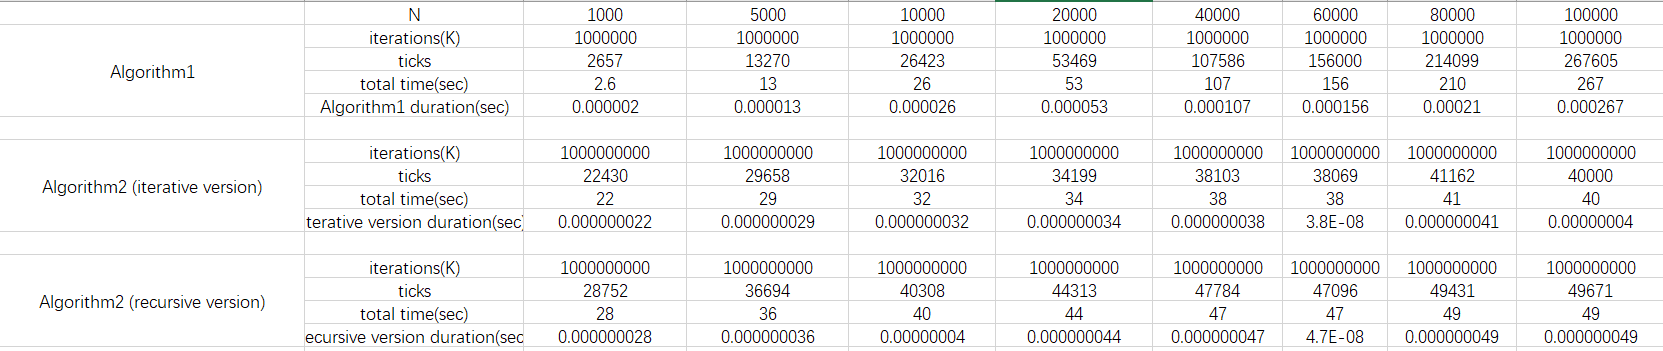
\includegraphics[width=0.99\textwidth]{result.png}
\caption{result}
\end{figure}
\par Since the running time of algorithm 1 is too large compared with that of algorithm 2, the n-runtime line graph of iterative version and recursive version of algorithm 2 is shown below
\begin{figure}[H]
\centering
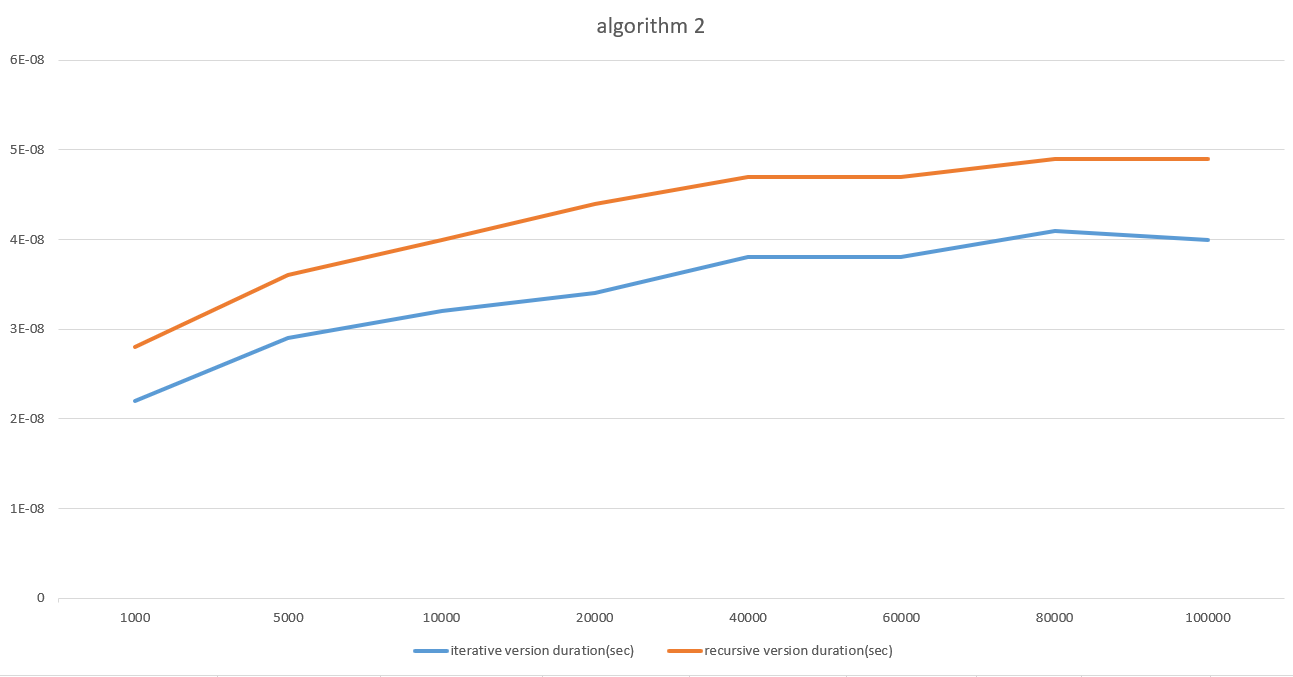
\includegraphics[width=0.99\textwidth]{algorithm2_result.png}
\caption{algorithm2 result}
\end{figure}
\par The following figure is the n-runtime diagram obtained by drawing the running time of two versions of algorithm 1 and algorithm 2 in the same line graph
\begin{figure}[H]
\centering
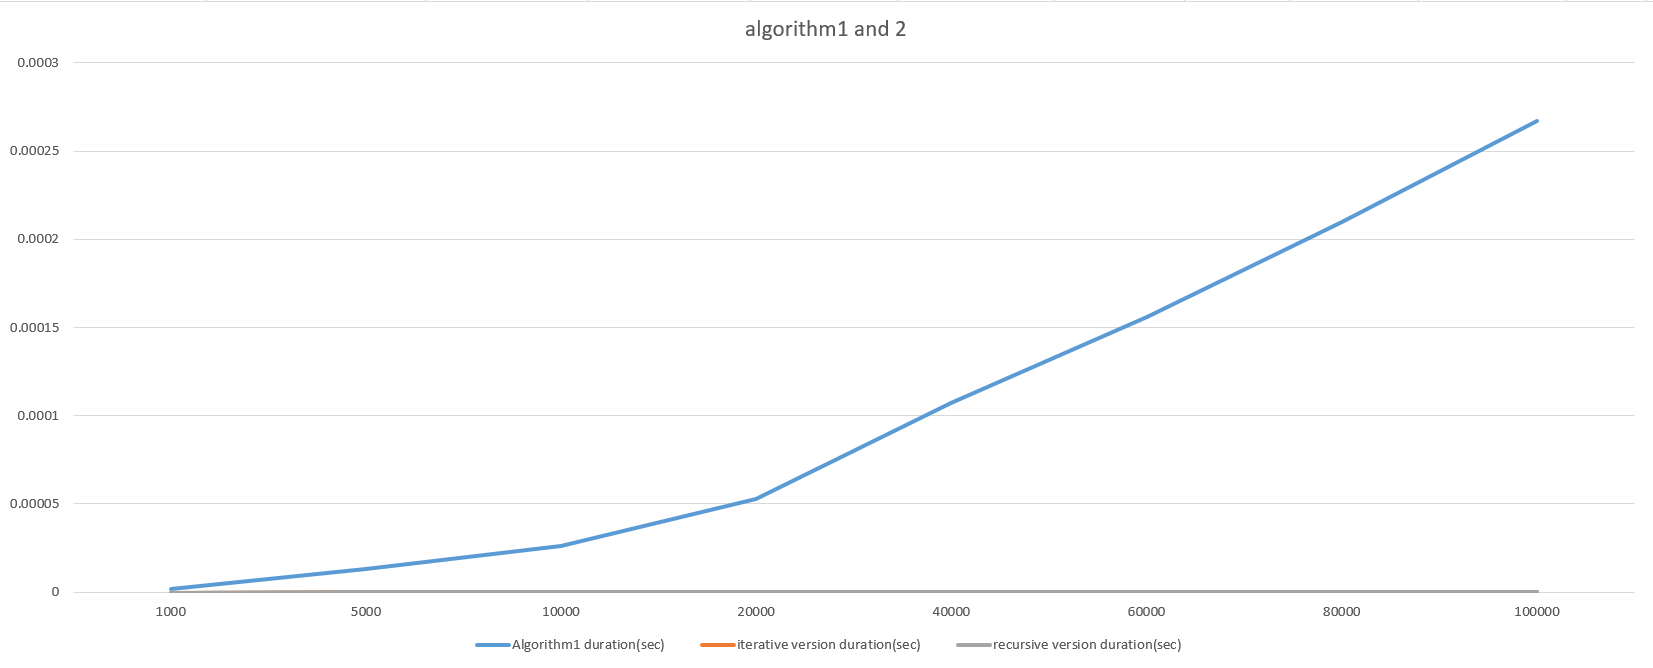
\includegraphics[width=0.99\textwidth]{algorithm1 and 2 result.png}
\caption{algorithm1 and 2 result}
\end{figure}
\par From the line graph, we can see that the running time of algorithm 1 is much longer than that of algorithm 2, and the running time of the two versions of algorithm 2 is almost the same

\section{Declaration}
I  hereby   declare   that   all   the   work   done   in   this   project   titled "POW" is of my independent effort.

\end{document}






好看的颜色 [HTML] 淡蓝色 CBF5FB
>{\columncolor[HTML]{AAACED}} 列背景颜色
\rowcolor, \cellcolor 行背景、单元背景颜色
